\documentclass[11pt,a4paper]{article}
\usepackage[utf8]{inputenc}
\usepackage[T1]{fontenc}
\usepackage[polish]{babel}
\usepackage[margin=2.4cm]{geometry}
\usepackage{graphicx}
\usepackage{booktabs}
\usepackage{amsmath,amssymb}
\usepackage{float}
\usepackage{xcolor}
\usepackage{listings}
\usepackage{caption}
\usepackage[hidelinks]{hyperref}

\captionsetup{font=small,labelfont=bf}

% --- listings: Python + polskie znaki ---
\definecolor{kod_tlo}{RGB}{247,247,247}
\definecolor{kod_kom}{RGB}{0,128,0}
\definecolor{kod_str}{RGB}{170,40,40}
\definecolor{kod_kw}{RGB}{0,60,170}
\lstset{
  language=Python, basicstyle=\ttfamily\footnotesize,
  backgroundcolor=\color{kod_tlo}, commentstyle=\color{kod_kom},
  stringstyle=\color{kod_str}, keywordstyle=\color{kod_kw}\bfseries,
  showstringspaces=false, breaklines=true, frame=single, framerule=0pt,
  xleftmargin=6pt, xrightmargin=6pt, aboveskip=8pt, belowskip=8pt,
  literate={ą}{{\k{a}}}1 {ć}{{\'c}}1 {ę}{{\k{e}}}1 {ł}{{\l{}}}1 {ń}{{\'n}}1
           {ó}{{\'o}}1 {ś}{{\'s}}1 {ź}{{\'z}}1 {ż}{{\.z}}1
           {Ą}{{\k{A}}}1 {Ć}{{\'C}}1 {Ę}{{\k{E}}}1 {Ł}{{\L{}}}1 {Ń}{{\'N}}1
           {Ó}{{\'O}}1 {Ś}{{\'S}}1 {Ź}{{\'Z}}1 {Ż}{{\.Z}}1 {°}{{$^\circ$}}1
}

\title{}
\begin{document}

% ===================== strona tytułowa =====================
\begin{titlepage}
\centering
{\large Politechnika Warszawska\\
Wydział Elektroniki i Technik Informacyjnych\\
kierunek: Automatyka i Robotyka\par}
\vspace{1cm}
{\large przedmiot: \textbf{Metody Identyfikacji}\par}
\vfill
{\LARGE\bfseries Predykcja zapchania młyna węglowego\\[4pt]
w elektrociepłowni na podstawie\\[4pt]
danych procesowych\par}
\vspace{1.2cm}
{\large analiza identyfikacyjna obiektu i porównanie modeli\\
wczesnego ostrzegania\par}
\vfill
{\large\textbf{Jakub Wróblewski}\\[2pt]
\textbf{Mateusz Smardzewski}\par}
\vspace{1.5cm}
{\large Warszawa, czerwiec 2026\par}
\end{titlepage}

\tableofcontents
\newpage

% ===================== 1 =====================
\section{Wstęp i cel projektu}

Zespoły młynowe (potocznie nazywane także kruszarkami węgla) są jednym
z~najbardziej awaryjnych elementów kotłów pyłowych. Zapchanie młyna ---
nadmierne nagromadzenie węgla w~komorze mielenia i~pyłoprzewodach --- prowadzi
do gwałtownego wzrostu mocy napędu, utraty wentylacji, a~w~skrajnym przypadku
do awaryjnego odstawienia młyna i~ograniczenia mocy bloku. Celem projektu jest
zbadanie, czy na podstawie standardowych, minutowych danych procesowych
z~systemu DCS można \emph{przewidzieć} nadchodzące zapchanie z~wyprzedzeniem
pozwalającym obsłudze na reakcję (odciążenie młyna), zanim zadziała automatyka
zabezpieczeniowa.

Projekt realizuje pełny tok postępowania identyfikacyjnego:
\begin{enumerate}
  \item analizę eksploatacyjnych danych pomiarowych obiektu (bez eksperymentu czynnego),
  \item identyfikację charakterystyk obiektu: charakterystyki statycznej,
        odpowiedzi skokowej toru regulacji (model FOPDT) oraz rekurencyjną
        identyfikację modelu ARX z~dyskusją ograniczeń identyfikacji
        w~zamkniętej pętli regulacji,
  \item interpretację zapchania jako \emph{dryfu parametrów obiektu}
        (spadku wzmocnienia statycznego kanału wentylacji),
  \item budowę i~porównanie modeli predykcyjnych: reguły fizycznej, modelu
        gradient boosting (LightGBM) oraz --- jako świadomego kontrprzykładu ---
        sieci neuronowych (MLP, LSTM),
  \item ocenę zdarzeniową jakości predykcji (wykrywalność epizodów, czas
        wyprzedzenia, częstość fałszywych alarmów).
\end{enumerate}

% ===================== 2 =====================
\section{Obiekt i dane pomiarowe}

\subsection{Zespół młynowy jako obiekt}

Analizowany blok wyposażony jest w~cztery zespoły młynowe MW1--MW4 (młyny
wentylatorowe). Węgiel podawany jest podajnikiem o~regulowanej prędkości,
mielony i~jednocześnie transportowany strumieniem powietrza wytwarzanym przez
wentylator młynowy. O~punkcie pracy decydują dwa tory regulacji (UAR):
\begin{itemize}
  \item \textbf{tor wentylacji}: regulator utrzymuje zadany przepływ mieszanki
        przez młyn, sterując kierownicą (łopatkami kierującymi) wentylatora,
  \item \textbf{tor temperatury mieszanki pyłowo-powietrznej}: regulator
        utrzymuje zadaną temperaturę za młynem, mieszając powietrze gorące
        i~zimne (klapy).
\end{itemize}

\subsection{Dane}

Dostępne dane obejmują okres 1--27 lutego 2026 (26~dni) z~próbkowaniem
1~minuta: po $37\,440$ próbek na młyn, ok.\ 38~sygnałów na młyn (tagi KKS),
oraz pliki pomocnicze (sygnały ogólnokotłowe, KPI kotła, lista punktów
pomiarowych, zrzuty ekranów DCS). Kluczowe wykorzystywane sygnały zestawiono
w~tabeli~\ref{tab:sygnaly}.

\begin{table}[H]
\centering\small
\caption{Najważniejsze sygnały zespołu młynowego (przykład dla MW1).}
\label{tab:sygnaly}
\begin{tabular}{lll}
\toprule
tag KKS & nazwa robocza & jednostka \\
\midrule
401HFC10AJ001XQ50:av & moc silnika młyna & kW \\
401HFB10AF001XQ51:av & prędkość podajnika węgla & \% \\
401HFB10AF001XQ50:av & prąd podajnika węgla & A \\
401HFE10DF201:me / :spa / :pos & wentylacja: pomiar / zadana / sterowanie & kNm$^3$/h, \% \\
401HFE10AA401:pos & położenie kierownicy wentylatora & \% \\
401HHE10FT950:av & temperatura mieszanki za młynem & $^\circ$C \\
401HHE10DT901:spa / :pos & temperatura mieszanki: zadana / sterowanie & $^\circ$C, \% \\
401HFE11AA401:pos / 401HFE12AA401:pos & klapa powietrza gorącego / zimnego & \% \\
401HFC10CP201:av & ciśnienie w~młynie & kPa \\
\bottomrule
\end{tabular}
\end{table}

Przygotowanie danych wymagało obsłużenia kilku pułapek typowych dla eksportów
przemysłowych: kodowania cp1250, braków zapisanych jako \texttt{N\_A},
a~przede wszystkim \emph{mieszanych formatów czasu w~obrębie jednego pliku}
(\texttt{dd.mm.yyyy HH:MM} oraz ISO~8601). Znaczniki czasu parsowano
dwuprzebiegowo (listing~\ref{lst:loader}); naiwne użycie automatycznej
detekcji formatu prowadziło do cichego przestawienia dnia z~miesiącem.

\begin{lstlisting}[caption={Dwuprzebiegowe parsowanie znaczników czasu (\texttt{src/loader.py}).},label={lst:loader}]
# pliki zawierają mieszane formaty czasu (dd.mm.yyyy HH:MM oraz ISO),
# dlatego parsujemy dwuprzebiegowo zamiast zgadywać dayfirst
t_iso = pd.to_datetime(df[tcol], format="ISO8601", errors="coerce")
t_pl  = pd.to_datetime(df[tcol], format="%d.%m.%Y %H:%M", errors="coerce")
df[tcol] = t_iso.fillna(t_pl)
if df[tcol].isna().any():
    raise ValueError(f"nierozpoznane znaczniki czasu w {path.name}")
\end{lstlisting}

% ===================== 3 =====================
\section{Analiza identyfikacyjna obiektu}

\subsection{Charakterystyka statyczna kanału kierownica\,$\to$\,przepływ}

Dla każdej minuty pracy młyna dysponujemy punktem pracy $(u, y)$, gdzie $u$ ---
położenie kierownicy [\%], $y$ --- przepływ wentylacji [kNm$^3$/h].
Rysunek~\ref{fig:charakterystyka} przedstawia chmurę punktów pracy MW3
z~podziałem na stan zdrowy oraz okna 60~minut przed epizodami zapchania.
W~stanie zdrowym charakterystyka jest monotoniczna i~nasyca się łagodnie;
przed zapchaniem punkty pracy przesuwają się w~prawo i~w~dół --- ten sam
przepływ wymaga znacznie większego otwarcia kierownicy, aż do pracy na
ograniczeniu $u=100\%$ przy malejącym $y$. Jest to obraz \emph{spadku
wzmocnienia statycznego} obiektu wskutek rosnącego oporu przepływu.

\begin{figure}[H]
\centering
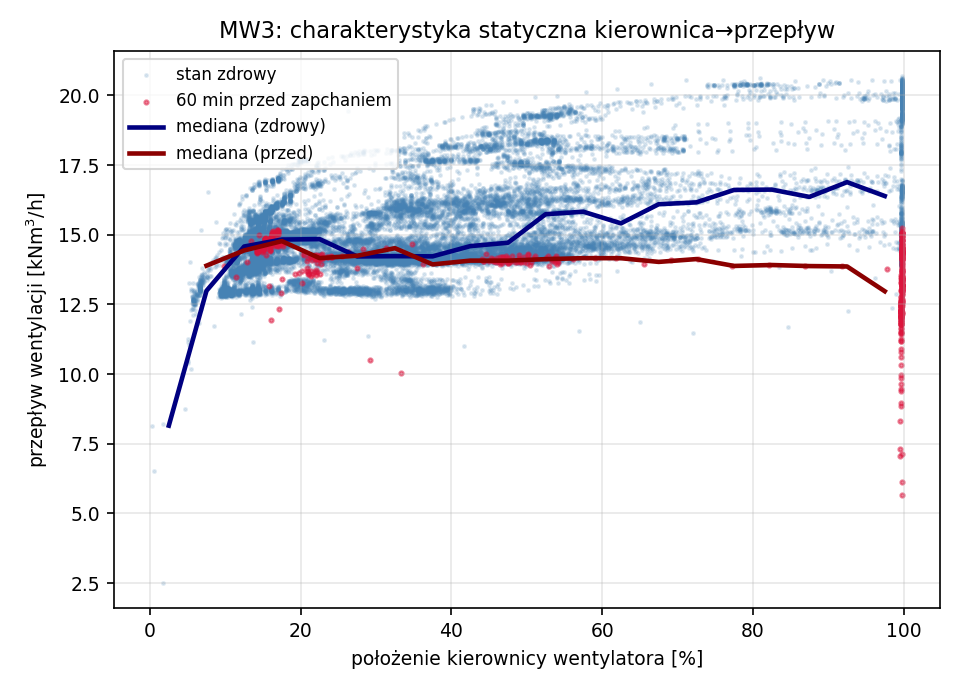
\includegraphics[width=0.78\textwidth]{fig/identyfikacja_charakterystyka_MW3.png}
\caption{MW3: charakterystyka statyczna kierownica$\to$przepływ wyznaczona
z~punktów pracy. Czerwone punkty: 60~min przed epizodami zapchania.}
\label{fig:charakterystyka}
\end{figure}

Jako odporny, punktowy estymator wzmocnienia statycznego przyjęto
\emph{drożność}
\begin{equation}
  k(t) \;=\; \frac{y(t)}{u(t)} \qquad
  \left[\tfrac{\mathrm{kNm^3/h}}{\%}\right],
  \label{eq:droznosc}
\end{equation}
której medianowe wartości zestawiono w~tabeli~\ref{tab:droznosc}. Spadek
drożności przed zapchaniem o~45--83\% stanowi fizyczną podstawę całego układu
wczesnego ostrzegania.

\begin{table}[H]
\centering\small
\caption{Mediana drożności $k$ (wygładzonej medianą 30~min) w~stanie zdrowym
i~w~oknach 60~min przed epizodami.}
\label{tab:droznosc}
\begin{tabular}{lccc}
\toprule
młyn & $k$ --- stan zdrowy & $k$ --- przed zapchaniem & spadek \\
\midrule
MW3 & 0{,}506 & 0{,}277 & $-45\%$ \\
MW4 & 0{,}917 & 0{,}152 & $-83\%$ \\
\bottomrule
\end{tabular}
\end{table}

\subsection{Odpowiedź skokowa i~model FOPDT toru temperatury}

Dane pochodzą z~normalnej eksploatacji (identyfikacja bierna), nie można więc
zadawać pobudzeń. Przeszukano jednak przebiegi wartości zadanych pod kątem
\emph{naturalnych skoków} z~plateau przed i~po zmianie. Wartość zadana
wentylacji zmienia się wyłącznie rampami (pochodzi z~układu obciążenia bloku),
natomiast wartość zadana temperatury mieszanki jest zmieniana przez operatora
skokowo --- znaleziono po kilkanaście czystych skoków ($|\Delta u|\ge 1\,^\circ$C,
stabilne plateau 10~min przed i~40~min po, brak wysycenia regulatora).

Znormalizowane odpowiedzi $\Delta y/\Delta u$ uśredniono i~dopasowano
metodą najmniejszych kwadratów model inercyjny pierwszego rzędu
z~opóźnieniem (FOPDT):
\begin{equation}
  G(s) \;=\; \frac{K\,e^{-sL}}{Ts+1},
  \qquad
  y(t) \;=\; K\!\left(1 - e^{-(t-L)/T}\right)\!\cdot\!\mathbf{1}(t\!\ge\!L).
  \label{eq:fopdt}
\end{equation}
Wyniki (tab.~\ref{tab:fopdt}, rys.~\ref{fig:skok}) opisują tor
\emph{zamkniętej} pętli regulacji temperatury: dla MW3 wzmocnienie statyczne
$K\approx 1$ oznacza poprawne nadążanie za wartością zadaną, a~stała czasowa
$T\approx 23$~min --- wolną dynamikę toru cieplnego (mieszanie powietrza,
pojemność cieplna młyna). Charakterystyczna jest mała wartość opóźnienia
czystego $L\approx 1$~min, zgodna z~transportem mieszanki przez młyn.

\begin{table}[H]
\centering\small
\caption{Parametry FOPDT odpowiedzi toru regulacji temperatury mieszanki
na skok wartości zadanej.}
\label{tab:fopdt}
\begin{tabular}{lcccc}
\toprule
młyn & liczba skoków & $K$ [--] & $T$ [min] & $L$ [min] \\
\midrule
MW3 & 15 & 1{,}01 & 22{,}7 & 1{,}0 \\
MW4 & 15 & 0{,}82 & 6{,}8 & 0{,}4 \\
\bottomrule
\end{tabular}
\end{table}

\begin{figure}[H]
\centering
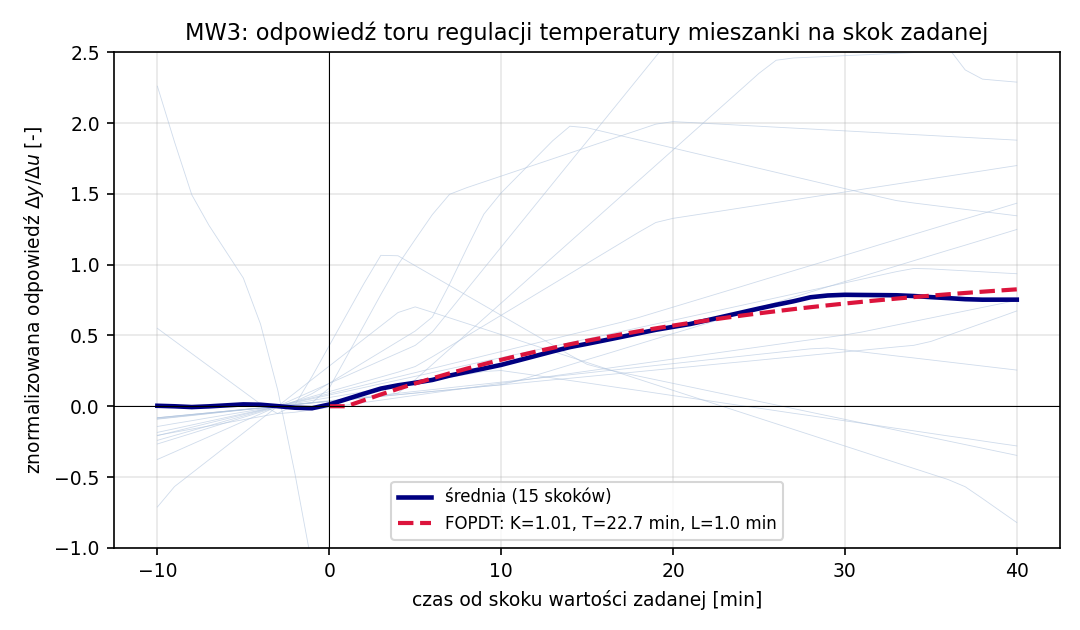
\includegraphics[width=0.8\textwidth]{fig/identyfikacja_skok_MW3.png}
\caption{MW3: uśredniona odpowiedź toru regulacji temperatury mieszanki na
skok wartości zadanej oraz dopasowany model FOPDT. Cienkie linie ---
pojedyncze skoki (zakłócenia eksploatacyjne).}
\label{fig:skok}
\end{figure}

Rozrzut pojedynczych odpowiedzi (cienkie linie) ilustruje koszt identyfikacji
biernej: pojedynczy ,,eksperyment'' jest silnie zakłócony zmianami obciążenia,
dopiero uśrednienie kilkunastu skoków daje gładką odpowiedź.

\subsection{Rekurencyjna identyfikacja ARX i~problem pętli zamkniętej}

Do śledzenia zmian dynamiki kanału kierownica$\to$przepływ zastosowano model
ARX(1,1)
\begin{equation}
  y(t) \;=\; a\,y(t\!-\!1) + b\,u(t\!-\!1) + e(t),
  \qquad \hat{K}_{ARX} = \frac{\hat b}{1-\hat a},
\end{equation}
estymowany rekurencyjną metodą najmniejszych kwadratów (RLS) z~wykładniczym
zapominaniem $\lambda = 0{,}998$ (listing~\ref{lst:rls}).

\begin{lstlisting}[caption={RLS z zapominaniem (\texttt{src/identyfikacja.py}).},label={lst:rls}]
def rls_arx(u, y, lam=0.998):
    """ARX(1,1): y(t) = a*y(t-1) + b*u(t-1)."""
    theta = np.zeros(2); P = np.eye(2) * 1000.0
    for t in range(1, len(y)):
        phi = np.array([y[t-1], u[t-1]])
        k = P @ phi / (lam + phi @ P @ phi)
        theta = theta + k * (y[t] - phi @ theta)
        P = (P - np.outer(k, phi @ P)) / lam
\end{lstlisting}

Wynik (rys.~\ref{fig:dryf}, dolny panel) jest pouczający \emph{negatywnie}:
estymata $\hat K_{ARX}$ przyjmuje dla MW3 wartości ujemne przez ok.~20\%
czasu pracy. Jest to klasyczne obciążenie identyfikacji bezpośredniej
w~zamkniętej pętli regulacji: przy stałej wartości zadanej jedynym źródłem
zmienności są zakłócenia wyjścia, na które regulator odpowiada ruchem
sterowania w~przeciwfazie --- korelacja $u$--$y$ odzwierciedla wtedy
(odwrócony) regulator, a~nie obiekt. Wiarygodna estymata pojawia się tylko
w~okresach bogatszego pobudzenia (zmiany zadanej). W~tej sytuacji prosty
iloraz punktu pracy~\eqref{eq:droznosc} (środkowy panel) okazuje się
odporniejszym wskaźnikiem wzmocnienia statycznego i~to on --- a~nie
$\hat K_{ARX}$ --- został użyty jako cecha modeli predykcyjnych.

\begin{figure}[H]
\centering
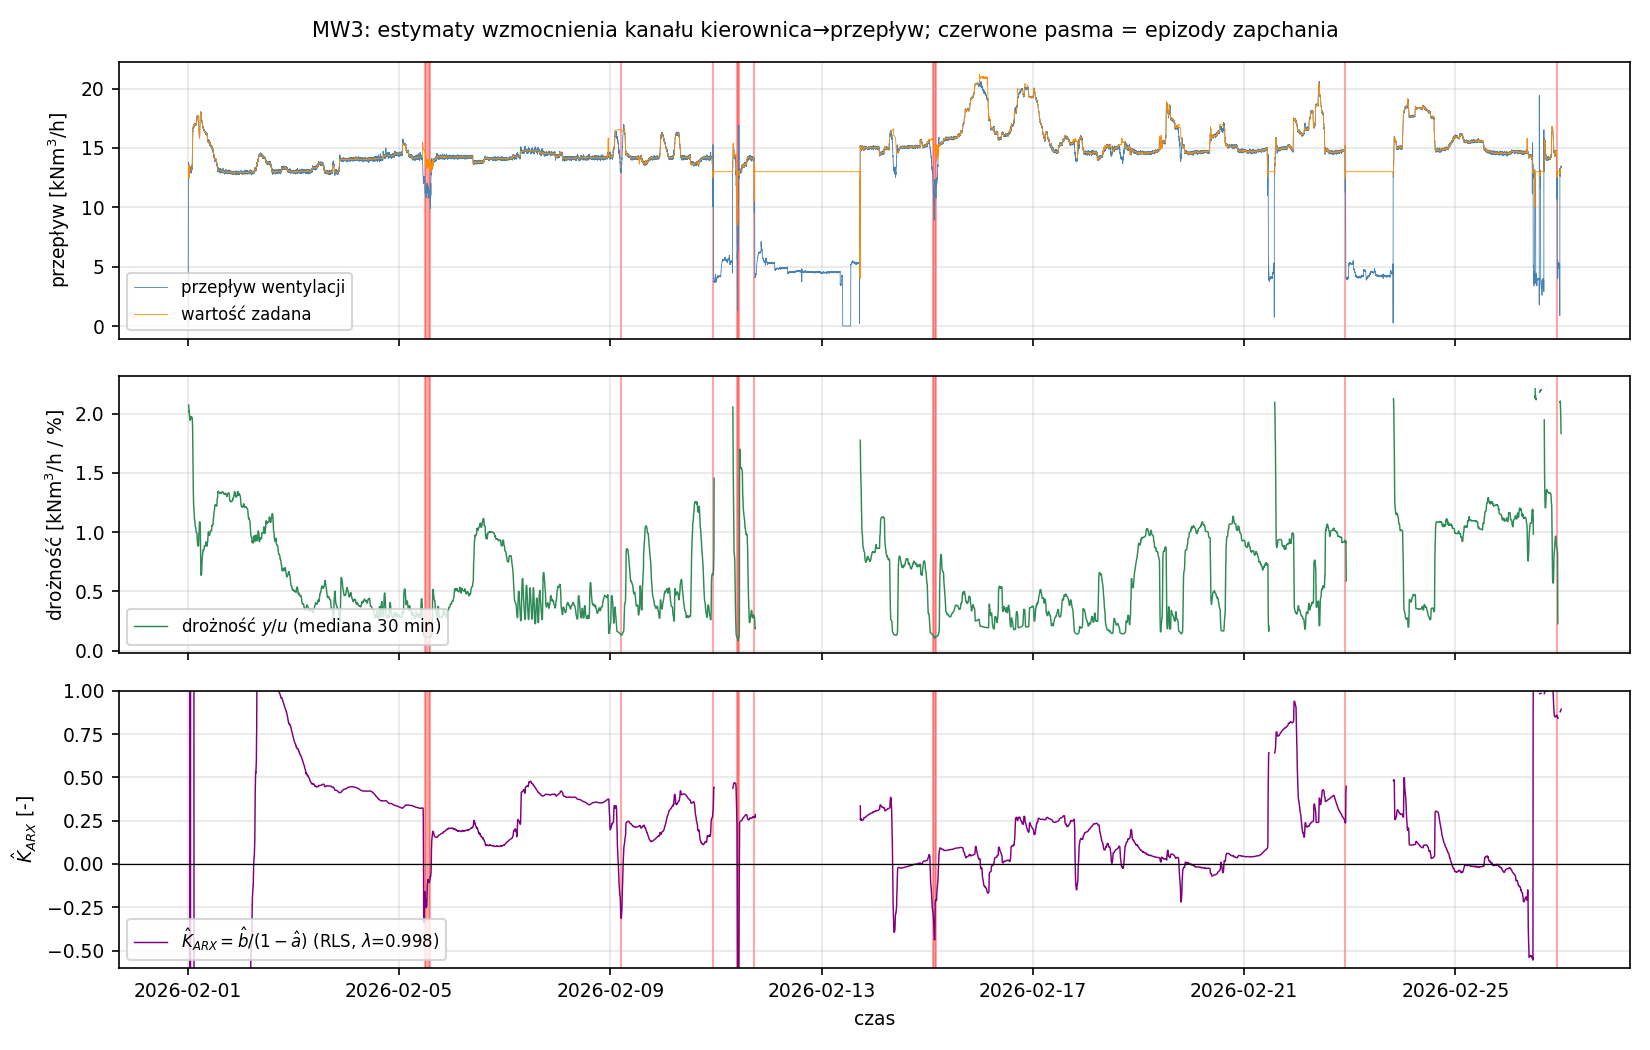
\includegraphics[width=\textwidth]{fig/identyfikacja_dryf_K_MW3.png}
\caption{MW3, luty 2026: przepływ wentylacji (góra), drożność $y/u$ (środek)
oraz estymata RLS wzmocnienia statycznego ARX (dół). Czerwone pasma ---
epizody zapchania. Widoczny spadek drożności przed epizodami oraz obciążenie
estymaty ARX w~pętli zamkniętej (wartości ujemne).}
\label{fig:dryf}
\end{figure}

\paragraph{Wniosek identyfikacyjny.} Zapchanie młyna jest obserwowalne jako
\emph{dryf parametru obiektu} --- spadek wzmocnienia statycznego kanału
wentylacji --- na długo przed wystąpieniem skutków (przeciążenia napędu,
utraty temperatury mieszanki). Zadanie predykcji zapchania można więc
sformułować jako detekcję zmiany parametrów obiektu na podstawie sygnałów
diagnostycznych.

% ===================== 4 =====================
\section{Definicja zdarzenia i~etykietowanie danych}

\subsection{Anatomia epizodu}

W~danych nie ma dziennika zdarzeń, dlatego epizody zapchania wyznaczono
sygnałowo i~zweryfikowano wizualnie. Rysunek~\ref{fig:anatomia} przedstawia
modelowy epizod (MW3, 15.02.2026): (I)~regulator wentylacji stopniowo otwiera
kierownicę aż do wysycenia 100\%; (II)~mimo wysycenia przepływ spada poniżej
wartości zadanej (deficyt), moc młyna rośnie, temperatura mieszanki spada
poniżej zadanej; (III)~automatyka cyklicznie odcina podajnik węgla
(przebieg piłokształtny), młyn się oczyszcza, kierownica schodzi z~ograniczenia.

\begin{figure}[H]
\centering
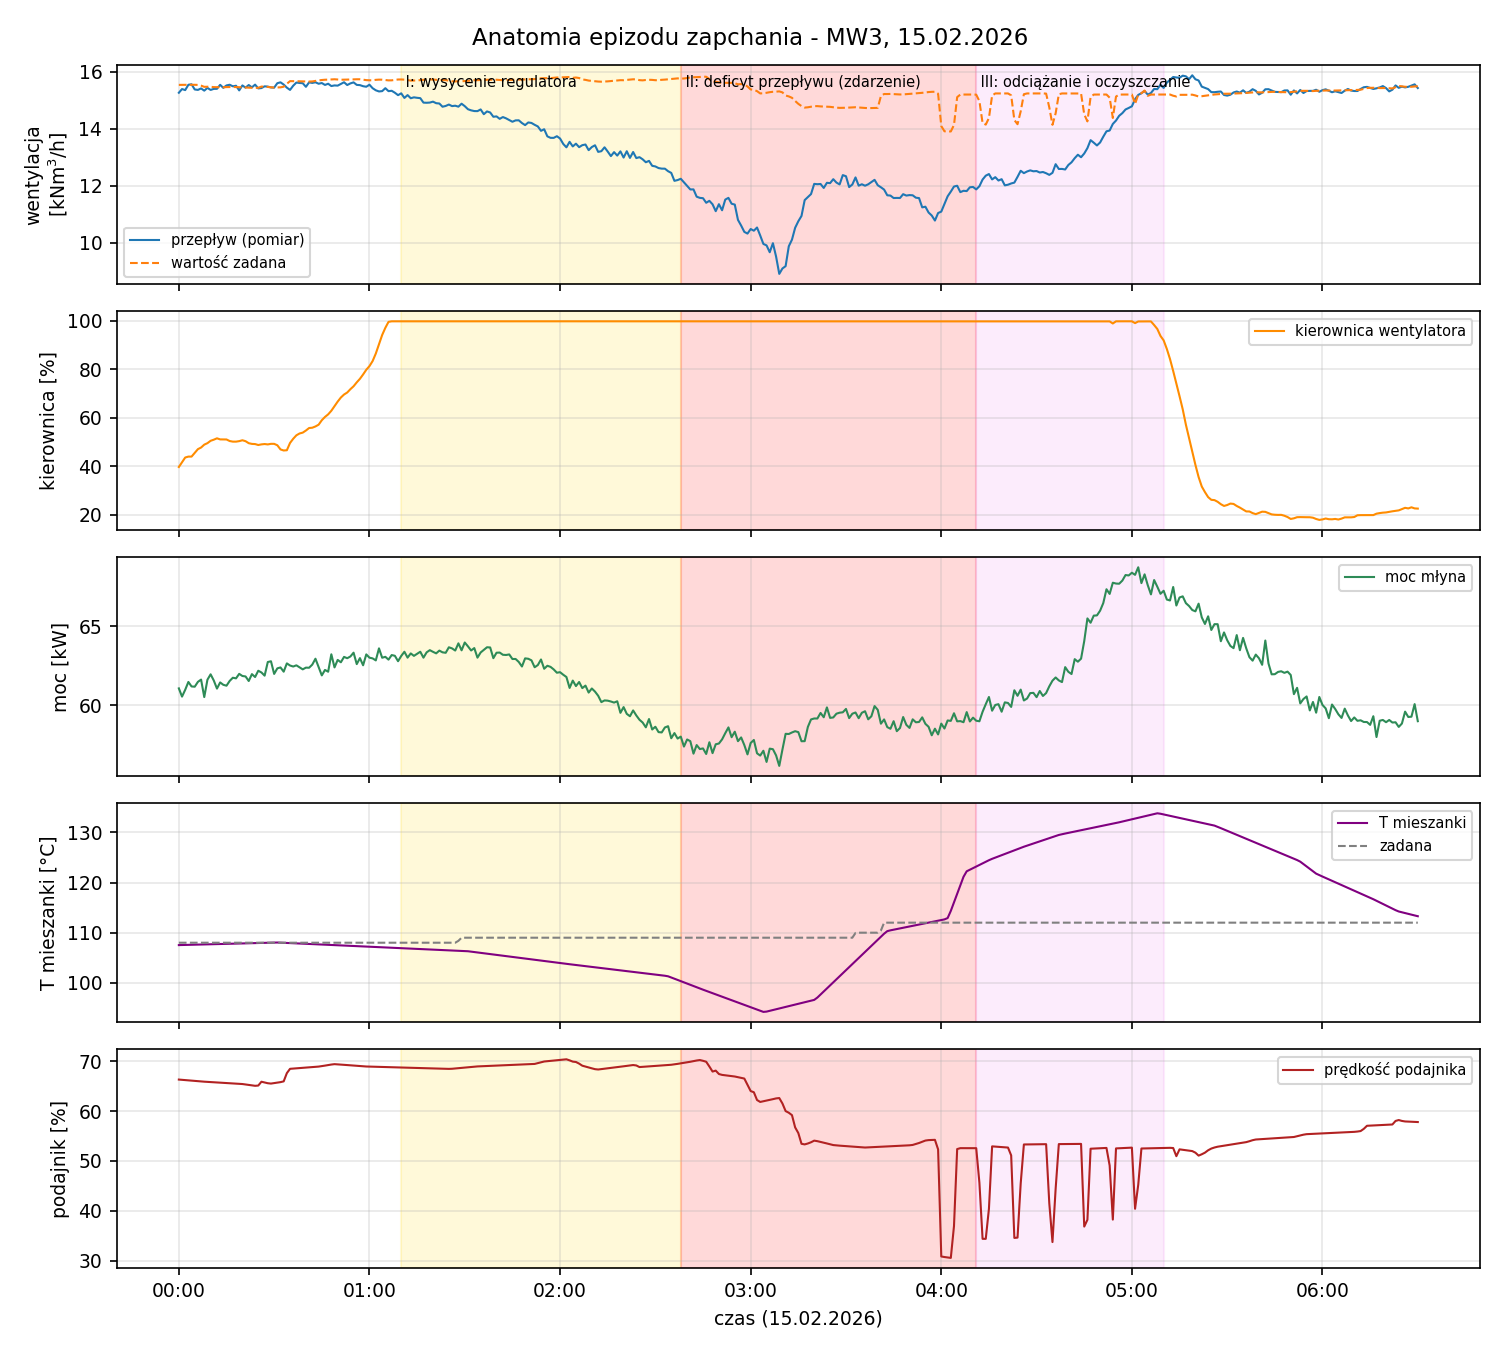
\includegraphics[width=0.92\textwidth]{fig/anatomia_zdarzenia.png}
\caption{Anatomia epizodu zapchania (MW3, 15.02.2026, 00:00--06:30).}
\label{fig:anatomia}
\end{figure}

\subsection{Sygnałowa definicja zdarzenia}

Zdarzenie ,,zapchanie'' zdefiniowano jako spełnienie --- w~czasie pracy młyna
(moc $>20$~kW) --- któregokolwiek z~warunków:
\begin{itemize}
  \item[\textbf{D1}] deficyt wentylacji
        $d(t) = \tfrac{y_{sp}(t)-y(t)}{y_{sp}(t)} > 0{,}2$
        nieprzerwanie przez $\ge 5$~min przy sterowaniu $\ge 98\%$,
  \item[\textbf{D2}] awaryjne odciążenie: spadek prędkości podajnika
        o~$\ge 25$~pkt w~$\le 3$~min, podczas gdy młyn nadal pracuje,
  \item[\textbf{D3}] przeciążenie: moc młyna powyżej kwantyla 99{,}5\%
        rozkładu w~pracy przy deficycie $>0{,}1$.
\end{itemize}
Minuty zdarzenia sklejano w~epizody (przerwa $<90$~min $\Rightarrow$ ten sam
epizod). Epizod uznano za \textbf{silny}, jeśli zawiera $\ge 3$~min warunku D1
--- ma wtedy fazę narastania, a~więc jest \emph{fizycznie przewidywalny}.
Pozostałe (nagłe odcięcia bez prekursorów) wyłączono z~uczenia i~oceny.
W~lutym 2026 zidentyfikowano \textbf{5~silnych epizodów} (tab.~\ref{tab:epizody})
oraz 7~mikrozdarzeń; wszystkie wystąpiły na MW3 i~MW4.

\begin{table}[H]
\centering\small
\caption{Silne epizody zapchania (etykiety do uczenia).}
\label{tab:epizody}
\begin{tabular}{lccc}
\toprule
młyn & początek & koniec & czas trwania \\
\midrule
MW3 & 05.02 11:54 & 05.02 14:16 & 143 min \\
MW3 & 09.02 04:39 & 09.02 05:00 & 22 min \\
MW3 & 11.02 09:40 & 11.02 10:15 & 36 min \\
MW3 & 15.02 02:38 & 15.02 04:11 & 94 min \\
MW4 & 19.02 18:15 & 19.02 19:19 & 65 min \\
\bottomrule
\end{tabular}
\end{table}

\subsection{Schemat etykietowania}

Cel predykcyjny sformułowano jako klasyfikację binarną: $y(t)=1$, jeśli silny
epizod rozpocznie się w~ciągu horyzontu $H=60$~min
(rys.~\ref{fig:etykiety}). Z~uczenia wyłączono: minuty postoju młyna, 60~min
po każdym rozruchu, czas trwania epizodów oraz 60~min rekonwalescencji po
nich. Zbiór uczący (4~młyny łącznie, cechy niezależne od numeru młyna)
liczy $131\,719$ minut, w~tym 300 pozytywnych (0{,}23\%).

\begin{figure}[H]
\centering
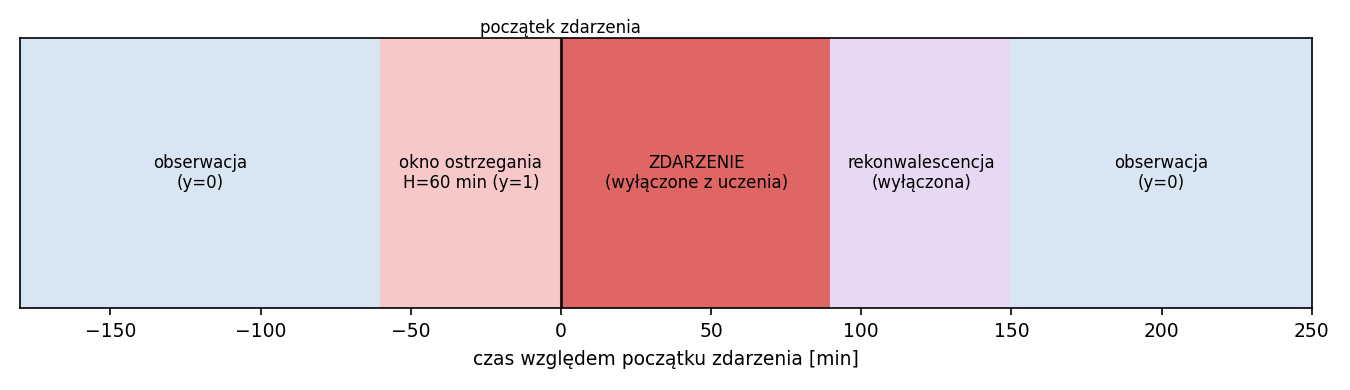
\includegraphics[width=0.95\textwidth]{fig/schemat_etykiet.png}
\caption{Schemat etykietowania względem początku zdarzenia.}
\label{fig:etykiety}
\end{figure}

% ===================== 5 =====================
\section{Modele predykcyjne}

\subsection{Cechy}

Zbudowano 39~cech liczonych wyłącznie z~przeszłości (bez wycieku przyszłości):
poziomy sygnałów, zmiany i~średnie kroczące w~oknach 15/30/60~min oraz cechy
fizyczne wynikające wprost z~analizy identyfikacyjnej
(listing~\ref{lst:cechy}): drożność~\eqref{eq:droznosc}, deficyt wentylacji,
energochłonność mielenia (moc na jednostkę strumienia węgla), liczba minut
wysycenia regulatora w~ostatniej godzinie, niestabilność mocy.

\begin{lstlisting}[caption={Kluczowe cechy fizyczne (\texttt{src/features.py}).},label={lst:cechy}]
deficyt  = (df["went_zadana"] - df["went_pomiar"]) / df["went_zadana"].clip(lower=1)
droznosc = df["went_pomiar"] / df["went_sterowanie"].clip(lower=1)
f["moc_na_wegiel"]   = df["moc_mlyna"] / df["podajnik_predkosc"].clip(lower=1)
f["t_miesz_odchylka"] = df["t_mieszanki"] - df["t_mieszanki_zadana"]
f["sat_min60"]    = (df["went_sterowanie"] >= 98).rolling(60).sum()
f["deficyt_min30"] = (deficyt > 0.10).rolling(30).sum()
f["moc_std30"]    = df["moc_mlyna"].rolling(30).std()
\end{lstlisting}

\subsection{Reguła fizyczna (poziom odniesienia)}

Najprostszy detektor zbudowano wprost z~fizyki zjawiska: alarm, gdy
w~ostatniej godzinie regulator wentylacji był wysycony przez $\ge 20$~min
\emph{i}~średni deficyt 15-minutowy przekracza 8\%. Reguła nie wymaga
uczenia i~stanowi poziom odniesienia dla modeli statystycznych.

\subsection{LightGBM}

Jako model główny wybrano gradient boosting (LightGBM) z~silną regularyzacją
(300~drzew o~maks. 15~liściach, \texttt{min\_child\_samples}=100,
podpróbkowanie wierszy i~kolumn, waga klasy pozytywnej ograniczona do~30).
Wybór wynika z~liczebności zdarzeń: przy 5~epizodach o~jakości decydują cechy,
a~nie pojemność modelu; boosting na cechach fizycznych jest interpretowalny
(ważności cech) i~trenuje się w~sekundy na CPU.

\subsection{Sieci neuronowe (kontrprzykład)}

Aby empirycznie zweryfikować hipotezę o~braku uzasadnienia dla uczenia
głębokiego przy tej liczbie zdarzeń, wytrenowano w~identycznym reżimie
walidacyjnym dwa warianty:
\begin{itemize}
  \item \textbf{MLP} (64--32, dropout 0{,}3) na \emph{tych samych} 39~cechach
        --- izoluje wpływ architektury od inżynierii cech,
  \item \textbf{LSTM} (32~jedn., głowica 16) na surowych sekwencjach
        $60\,\mathrm{min}\times 12$~sygnałów --- test, czy sieć sama
        ,,odkryje'' cechy z~surowych przebiegów (listing~\ref{lst:lstm}).
\end{itemize}

\begin{lstlisting}[caption={Architektura LSTM (\texttt{src/nn\_experiment.py}).},label={lst:lstm}]
class LSTMNet(nn.Module):
    def __init__(self, n_sig, hidden=32):
        super().__init__()
        self.lstm = nn.LSTM(n_sig, hidden, batch_first=True)
        self.head = nn.Sequential(nn.Linear(hidden, 16), nn.ReLU(), nn.Linear(16, 1))
    def forward(self, x):
        out, _ = self.lstm(x)
        return self.head(out[:, -1]).squeeze(-1)
\end{lstlisting}

Niezbalansowanie klas (0{,}23\% pozytywnych) obsłużono wagą klasy pozytywnej
w~funkcji straty (\texttt{BCEWithLogitsLoss(pos\_weight)}, ograniczenie
do~30) oraz --- dla LSTM --- podpróbkowaniem negatywów w~zbiorze uczącym
(wszystkie pozytywy zachowane).

% ===================== 6 =====================
\section{Metodyka oceny}

\paragraph{Walidacja.} Dane są szeregiem czasowym, więc zwykła walidacja
krzyżowa zawyżałaby wyniki (wyciek przez okna kroczące). Zastosowano
\emph{GroupKFold po dniach kalendarzowych}: (a)~wariant 5-krotny --- do
uczciwego porównania trzech modeli (koszt uczenia sieci), (b)~wariant
leave-one-day-out (27~foldów) --- do oceny modelu finalnego. Wszystkie
podawane predykcje są pozapróbkowe (out-of-fold).

\paragraph{Metryki minutowe.} PR-AUC (average precision) i~ROC-AUC liczone
na poziomie pojedynczych minut. Przy 0{,}23\% klasy pozytywnej losowy
klasyfikator ma PR-AUC $\approx 0{,}002$.

\paragraph{Metryki zdarzeniowe.} Z~punktu widzenia obsługi liczy się:
(a)~czy epizod został wykryty w~oknie ostrzegania (alarm $=$ co najmniej
3~kolejne minuty ze score $\ge$ progu), (b)~czas wyprzedzenia względem
początku zdarzenia, (c)~liczba fałszywych serii alarmowych na dobę pracy
młyna. Wyjścia modeli wygładzono medianą kroczącą 5~min.

% ===================== 7 =====================
\section{Wyniki}

\subsection{Porównanie modeli}

\begin{table}[H]
\centering\footnotesize
\caption{Porównanie modeli --- identyczna walidacja 5-fold po dniach,
próg alarmu 0{,}5. FA = fałszywe serie alarmowe na dobę i~młyn.
Reguła fizyczna oceniona na tym samym zbiorze; LODO = leave-one-day-out.}
\label{tab:wyniki}
\begin{tabular}{lccccc}
\toprule
model & PR-AUC & ROC-AUC & wykryte & wyprzedz. [min] & FA \\
\midrule
reguła fizyczna  & ---    & ---    & \textbf{5/5} & \textbf{48{,}8} & 0{,}074 \\
LightGBM (cechy) & 0{,}286 & 0{,}931 & 4/5 & 33{,}0 & \textbf{0{,}046} \\
MLP (cechy)      & \textbf{0{,}362} & 0{,}859 & 4/5 & 50{,}5 & 0{,}074 \\
LSTM (sekwencje) & 0{,}206 & \textbf{0{,}975} & 4/5 & 42{,}0 & 0{,}102 \\
\midrule
LightGBM, LODO (27 foldów)     & 0{,}359 & 0{,}953 & \textbf{5/5} & 30{,}0 & 0{,}056 \\
hybryda: LightGBM $\lor$ reguła, LODO & --- & --- & \textbf{5/5} & \textbf{51{,}0} & 0{,}093 \\
\bottomrule
\end{tabular}
\end{table}

\begin{figure}[H]
\centering
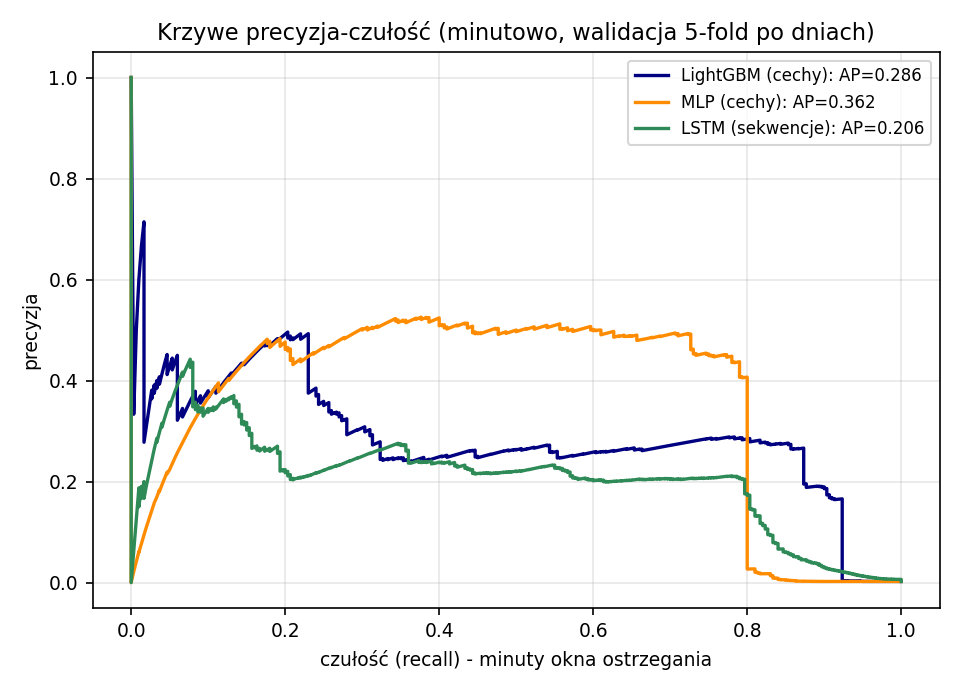
\includegraphics[width=0.72\textwidth]{fig/krzywe_pr.png}
\caption{Krzywe precyzja--czułość trzech modeli (minutowo, predykcje
pozapróbkowe, walidacja 5-fold po dniach).}
\label{fig:pr}
\end{figure}

\begin{figure}[H]
\centering
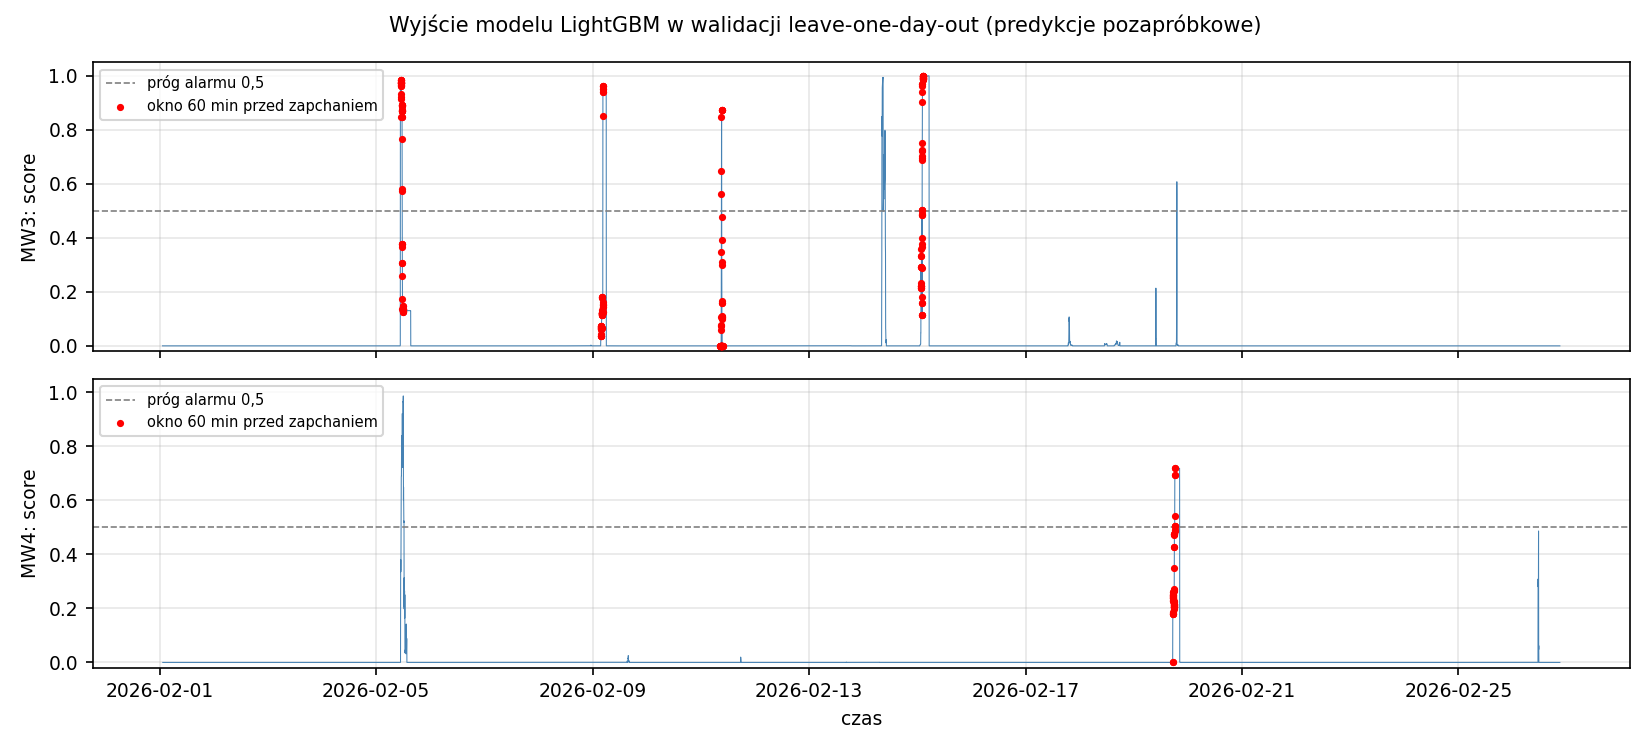
\includegraphics[width=\textwidth]{fig/score_oof.png}
\caption{Wyjście modelu LightGBM (walidacja leave-one-day-out) dla MW3 i~MW4.
Czerwone punkty --- minuty okien ostrzegania przed epizodami.}
\label{fig:score}
\end{figure}

Model finalny (LightGBM, walidacja leave-one-day-out, próg 0{,}5, alarm po
3~kolejnych minutach) wykrywa \textbf{5/5} silnych epizodów ze średnim
wyprzedzeniem \textbf{30~min} przy \textbf{0{,}056} fałszywej serii na dobę
i~młyn. Hybryda z~regułą fizyczną (alarm, gdy którykolwiek człon zgłasza)
wydłuża wyprzedzenie do \textbf{51~min} kosztem nieznacznego wzrostu liczby
fałszywych alarmów. Najważniejsze cechy modelu (rys.~\ref{fig:waznosci})
pokrywają się z~analizą identyfikacyjną: poziom i~trend przepływu, średnia
moc młyna, odchyłka temperatury mieszanki, liczba minut deficytu i~wysycenia.

\begin{figure}[H]
\centering
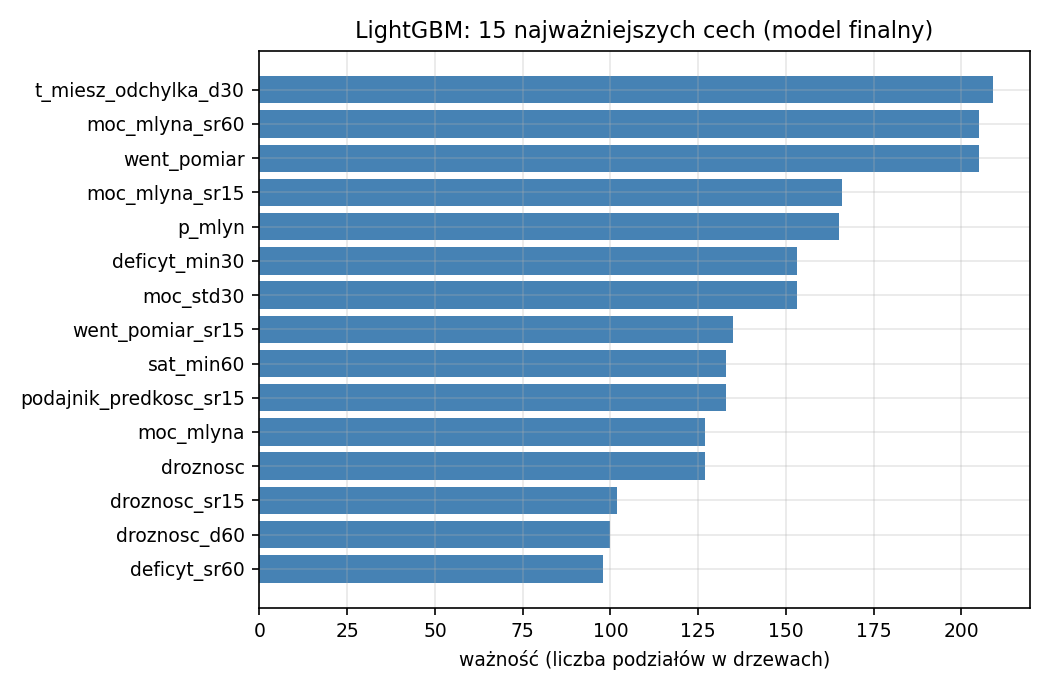
\includegraphics[width=0.74\textwidth]{fig/waznosci_cech.png}
\caption{Ważności cech finalnego modelu LightGBM.}
\label{fig:waznosci}
\end{figure}

\subsection{Sieci neuronowe --- analiza kontrprzykładu}

Tabela~\ref{tab:wyniki} pokazuje, że żaden z~wariantów sieci nie dominuje
spójnie: MLP ma najwyższe PR-AUC, ale najniższe ROC-AUC; LSTM odwrotnie ---
najwyższe ROC-AUC przy najniższym PR-AUC i~\emph{dwukrotnie} większej liczbie
fałszywych alarmów niż LightGBM. Zdarzeniowo wszystkie trzy modele wykrywają
te same 4/5 epizodów.

\begin{figure}[H]
\centering
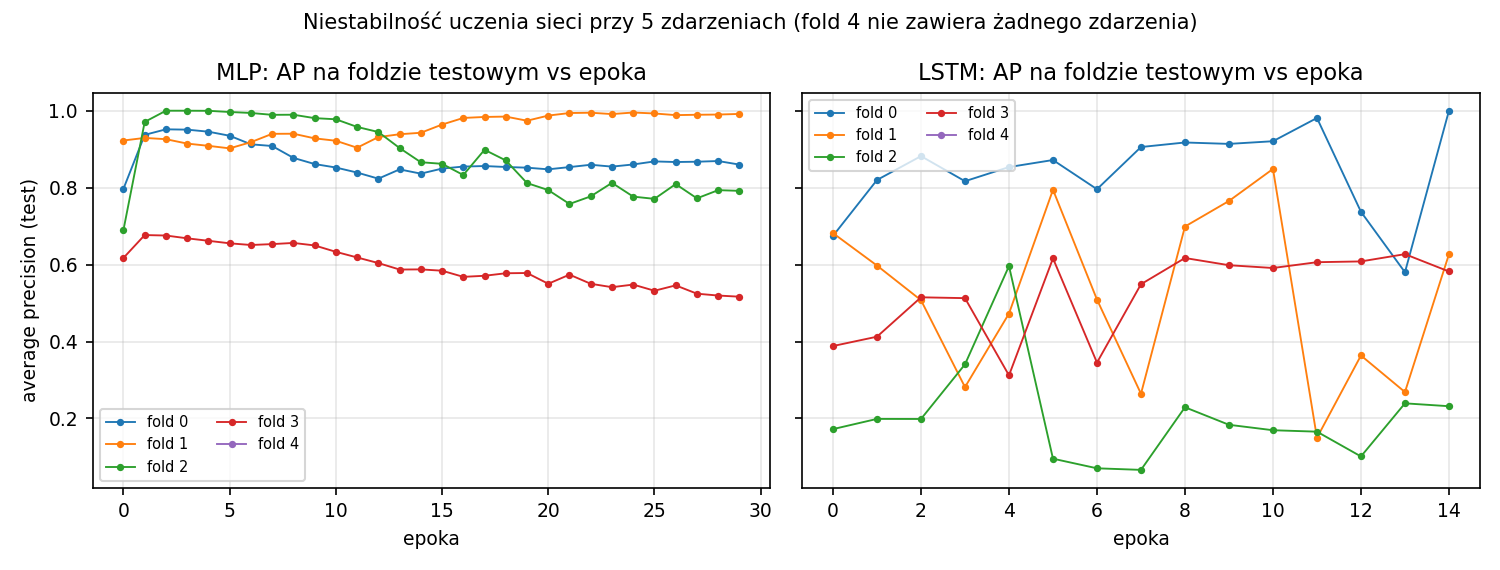
\includegraphics[width=\textwidth]{fig/krzywe_uczenia_nn.png}
\caption{Krzywe uczenia sieci: average precision na foldzie testowym po
każdej epoce. Fold~4 nie zawiera żadnego zdarzenia (AP nieokreślone).}
\label{fig:uczenie}
\end{figure}

Istotniejsza od średnich wyników jest \emph{niestabilność}
(rys.~\ref{fig:uczenie}): dla LSTM wynik na foldzie testowym oscyluje między
epokami w~zakresie 0{,}07--1{,}0 (fold~2: AP $=0{,}60$ w~epoce~4
i~$0{,}10$ w~epoce~5), a~dla MLP fold~3 wykazuje systematyczne przeuczanie.
Przy 5~zdarzeniach: (a)~nie istnieje sensowny zbiór walidacyjny do wyboru
epoki/architektury --- każda decyzja jest de~facto dopasowaniem do zbioru
testowego; (b)~różnice między modelami mieszczą się w~wariancji pojedynczego
epizodu; (c)~rozbieżność między AP liczonym osobno na foldach (0{,}5--1{,}0)
a~AP zbiorczym (0{,}2--0{,}36) ujawnia dodatkowo problem niekalibrowanych
score'ów między foldami. Wniosek: \textbf{przy obecnej liczbie zdarzeń wybór
sieci neuronowej nie znajduje statystycznego uzasadnienia}, a~prostszy model
na cechach fizycznych jest preferowany także ze względu na interpretowalność
i~koszt wdrożenia. Sieci sekwencyjne (LSTM/TCN) mogą zyskać przewagę dopiero
przy zbiorze rzędu kilkudziesięciu--kilkuset epizodów (6--12~miesięcy danych
z~kilku bloków).

% ===================== 8 =====================
\section{Dyskusja}

\paragraph{Spójność wyników z~fizyką.} Wszystkie trzy niezależne spojrzenia
--- analiza identyfikacyjna (spadek wzmocnienia statycznego), reguła fizyczna
(wysycenie $+$ deficyt) i~ważności cech modelu --- wskazują ten sam mechanizm:
zapchanie rozwija się przez dziesiątki minut jako narastający opór przepływu
kompensowany przez regulator aż do wysycenia. To uzasadnia zaufanie do
modelu mimo małej liczby zdarzeń.

\paragraph{Ograniczenia.} (a)~Etykiety wyznaczono sygnałowo --- wymagają
potwierdzenia dziennikiem zdarzeń DCS; (b)~5~epizodów z~jednego miesiąca
i~dwóch młynów to studium wykonalności, nie walidacja produkcyjna;
(c)~mikrozdarzeń (nagłych odcięć bez fazy narastania) z~definicji nie da się
przewidzieć z~minutowych danych procesowych; (d)~identyfikacja przebiegała
w~zamkniętej pętli regulacji --- część charakterystyk (FOPDT) opisuje układ
regulacji, a~nie sam obiekt; pełna identyfikacja obiektu wymagałaby
eksperymentu czynnego.

\paragraph{Wdrożenie.} Model przelicza pojedynczą minutę w~milisekundach na
CPU. Proponowany układ: liczenie cech w~oknie kroczącym na strumieniu 1-min
z~DCS, alarm po 3~kolejnych minutach score $\ge 0{,}5$, równolegle reguła
fizyczna jako niezależny watchdog (hybryda --- najdłuższe wyprzedzenie).

% ===================== 9 =====================
\section{Wnioski}

\begin{enumerate}
  \item Zapchanie młyna węglowego jest w~danych procesowych obserwowalne jako
        \textbf{dryf wzmocnienia statycznego} kanału kierownica$\to$przepływ
        (spadek drożności o~45--83\%) na 1--2~h przed kulminacją zdarzenia.
  \item Tor regulacji temperatury mieszanki daje się opisać modelem FOPDT
        ($K\!\approx\!1$, $T\!\approx\!23$~min dla MW3) wyznaczonym
        z~naturalnych skoków wartości zadanej; bezpośrednia identyfikacja
        ARX w~pętli zamkniętej jest obciążona (ujemne estymaty wzmocnienia)
        i~wymaga ostrożnej interpretacji.
  \item Finalny model (LightGBM na 39~cechach fizycznych, walidacja
        leave-one-day-out) wykrywa \textbf{5/5} epizodów ze średnim
        wyprzedzeniem \textbf{30~min} przy \textbf{0{,}06} fałszywej serii
        na dobę i~młyn; hybryda z~regułą fizyczną wydłuża wyprzedzenie
        do~\textbf{51~min}.
  \item Eksperyment kontrolny z~sieciami neuronowymi (MLP, LSTM) potwierdził
        hipotezę: przy 5~zdarzeniach sieci nie dają spójnej przewagi, a~ich
        uczenie jest niestabilne --- o~jakości decyduje inżynieria cech
        zakorzeniona w~fizyce obiektu, nie pojemność modelu.
  \item Dalsze prace: potwierdzenie etykiet dziennikiem zdarzeń, wydłużenie
        horyzontu danych do 6--12~miesięcy, dołączenie sygnałów
        ogólnokotłowych (obciążenie, jakość węgla) oraz --- przy większej
        liczbie epizodów --- ponowna ocena modeli sekwencyjnych.
\end{enumerate}

\appendix
\section{Reprodukcja wyników}

Środowisko: Python~3.12 (WSL2 Ubuntu~24.04), pakiety \texttt{pandas},
\texttt{scikit-learn}, \texttt{lightgbm}, \texttt{torch} (CPU),
\texttt{scipy}, \texttt{matplotlib}. GPU nie jest wymagane. Kolejność
uruchamiania skryptów oraz strukturę projektu opisuje plik \texttt{README.md};
pełny kod źródłowy znajduje się w~katalogu \texttt{src/}, artefakty
(model, wyniki, ryciny) w~katalogu \texttt{work/}.

\end{document}
